\chapter{El Proyecto}

\section{Motivación}

En la actualidad existen pocos sistemas Aplicados en el ambito de la gestion en
el area de Medicina y los existentes suelen ser solo para areas especificas

\section{Descripci\'on del Proyecto}
INCOMPLETO


\section{Arquitectura de la Aplicacion}

Implementado en Python utilizando en Framework Django, utilizando el motor de bases
de datos PosgreSQL, funciona con una interfaz web por lo que se se accede al
mismo mediante un Navegador Web, Internamente maneja 2 Modulos principales
que son el  ``Modulo de Gestion de Turnos" y el ``Modulo de manejo de
Historia Clinica" , al ser un sistema web implementa un tercer modulo de manera
implicita que control de acceso mediante la definicion de Grupos Usuarios y
sus correspondientes permisos.

\section{Modulo Usuarios}

La gestion de usuarios es un proceso bastante comun en casi todos los sistemas,
muchos desarrolladores terminan programando funcionalidades de autenticacion 
una y otra ves a lo largo de los a\'nos y casi siempre funcionando de la misma 
manera. Django se penso para simplificar la vida no para complicarla, por eso
al ser una tarea bastante comun en casi todas las aplicaciones, viene incluido
un completo sistema de autenticacion que gestiona:

\begin{itemize}
    \item Usuarios
    \item Grupos
    \item Permisos
    \item Sessiones de Usuarios y Cookies
\end{itemize}

Aunque en cuanto a lo que se refiere manejo de sessiones es un completo sistema
solo maneja un peque\~no conjunto de datos por lo que hubo que estender mediante 
la adicion de un Modelo adicional para complementar la informacion de los 
usuarios.

\subsection{Modelos}

Aqui un diagrama con todos los modelos que componen el modulo Usuarios.

\begin{figure}[H]
    \centering
    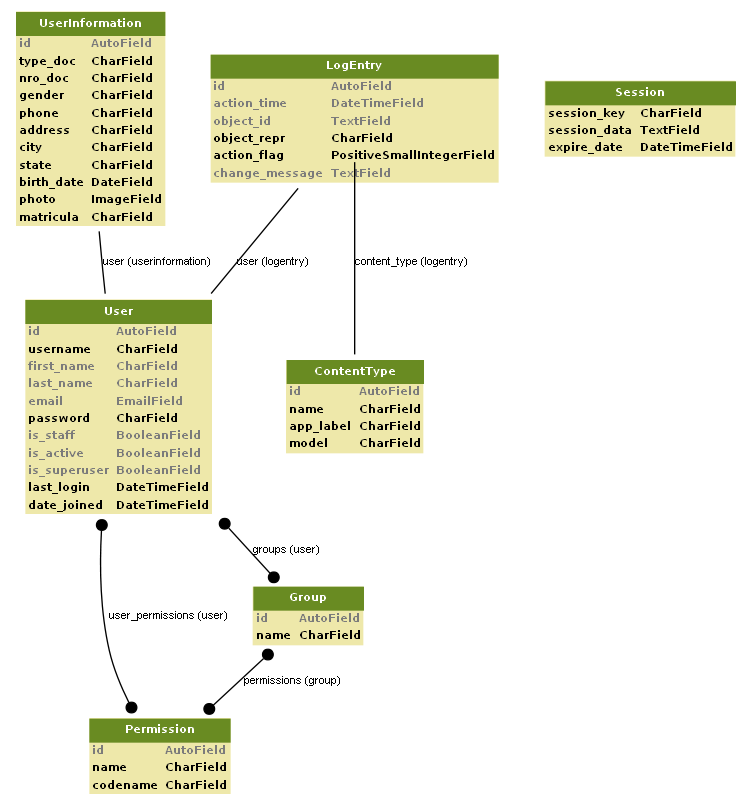
\includegraphics[scale=0.7]{resourse/auth.png}
    \caption{Modelo Historia Clinica Ministerio de Salud de La Nacion Pag 2}
    \label{fig:07}
\end{figure}

El unico modelo que fue necesario agregar es UserInformation el resto vienen
con Django. En Resumen aunque se podria haber desarrollado Un Modulo desde
 cero que gestione las sessiones de usuarios hubiese generado trabajo extra sin
 sentido.

\section{Modulo Gestion de Turnos}

\section{Modulo Historia Clinica}

\section{Elecci\'on de la metodolog\'ia de Programaci\'on}

